\chapter{Testing Results}
%TC:ignore

\label{appendix:test_results}
This appendix chapter shows the different sections of the application that has been tested and the test outcomes.


\section{Unit tests} \label{test:unit}
\subsection{Binarise image}
\begin{figure}[H]
  \centering
  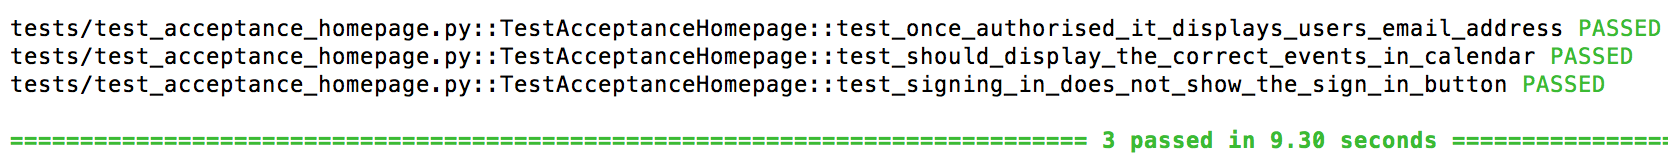
\includegraphics[width=\textwidth]{images/test_acceptance_homepage}
  \caption{Acceptance test being conducted for the homepage, to ensure that the homepage displays the correct content.}
  \label{fig:acceptance_homepage}
\end{figure}

\section{Acceptance tests} \label{tests:acceptance}
\label{appendix:acceptance}
The following section displays visual representation of the acceptance tests being executed, and their overall status.

\subsection{Add meta-data}

\begin{figure}[H]
  \centering
  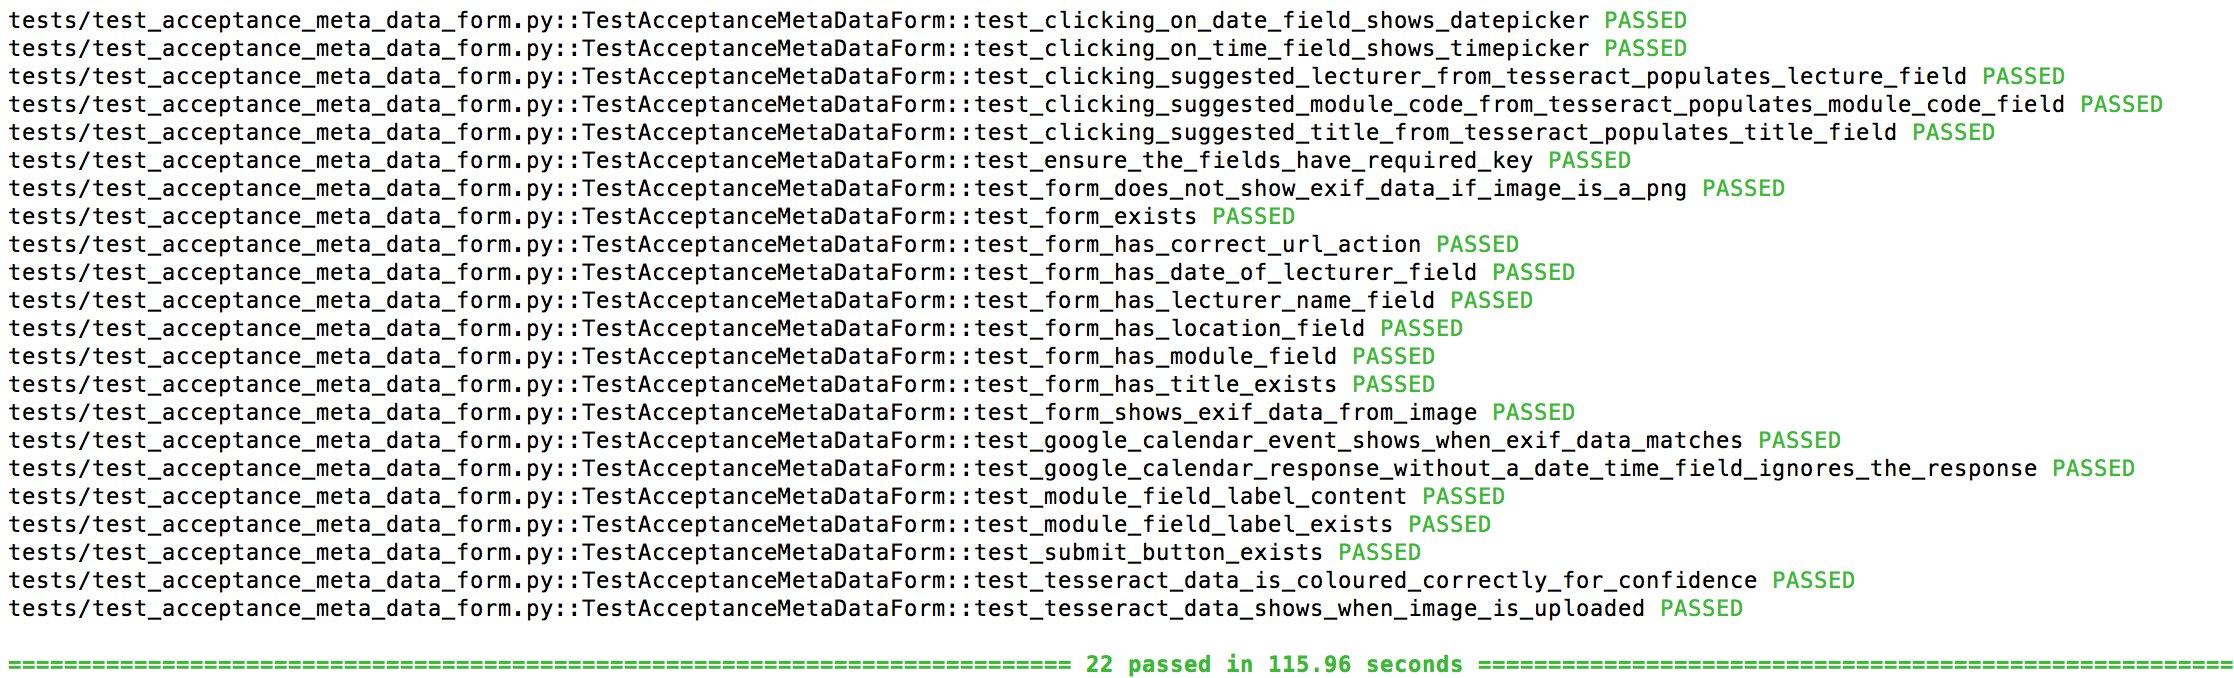
\includegraphics[width=\textwidth]{images/test_acceptance_meta_data_form}
  \caption{Acceptance test being performed to ensure that meta-data can be added to the correct note.}
  \label{fig:acceptance_add_meta_data}
\end{figure}

\subsection{Viewing all the notes}

\begin{figure}[H]
  \centering
  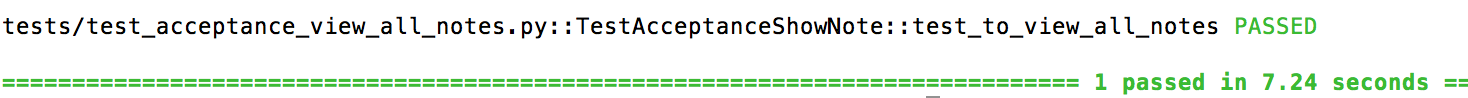
\includegraphics[width=\textwidth]{images/test_acceptance_view_notes}
  \caption{Acceptance test being conducted to ensure that all the notes can be viewed.}
  \label{fig:acceptance_view_note}
\end{figure}


\section{Integration tests}
\label{appendix:integration_tests}

\subsection{Add and edit meta data}
\begin{figure}[H]
  \centering
  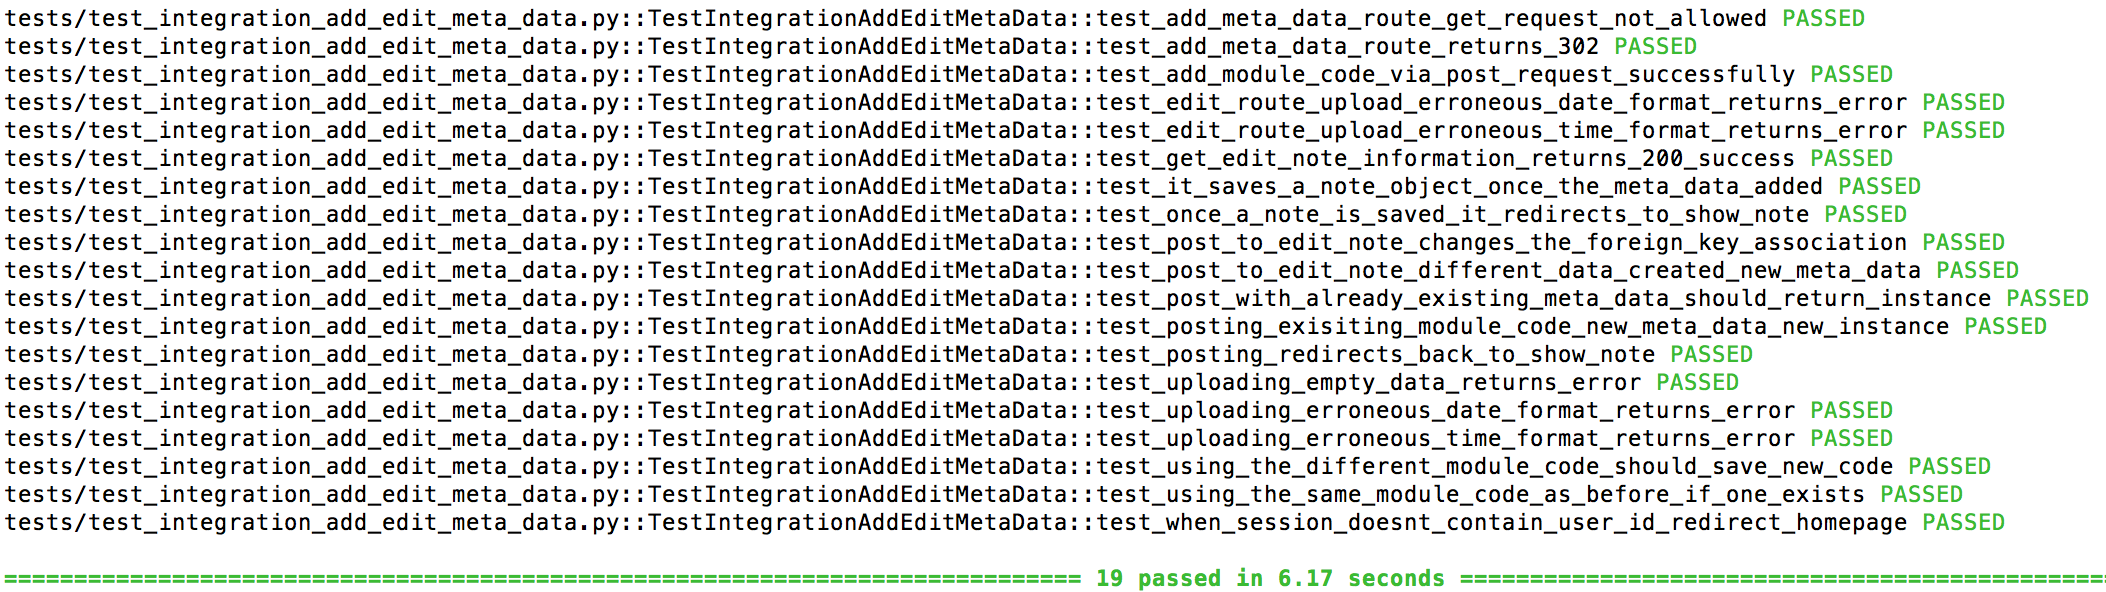
\includegraphics[width=\textwidth]{images/test_integration_add_edit_meta_data}
  \caption{Integration tests carried on the add and edit meta url to ensure the system worked well together.}
  \label{fig:integration_add_edit}
\end{figure}

\section{User study tests}
TODO
%TC:endignore 
